\section{Fonctionnement de l'application}

L'application fonctionne à l'aide du framework Swing de Java pour l'interface graphique.
Tout d'abord, l'application lance le menu principal qui permet d'indiquer le nom des deux joueurs 
avec un bouton Play pour lancer la partie (cf. \hyperref[f:menuPrincipal]{figure \ref{f:menuPrincipal}}). \medskip

\begin{figure}[H]
    \centering
    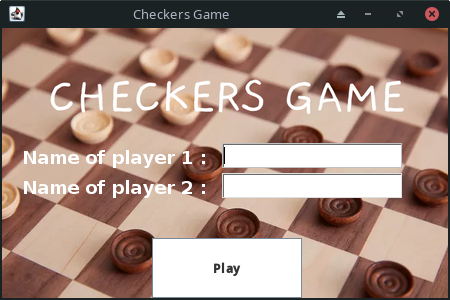
\includegraphics[width=0.8\columnwidth]{figures/mainMenu.png}
    \caption[Menu principal du jeu de dames]{Menu principal du jeu de dames}
    \label{f:menuPrincipal}
\end{figure}

Ensuite, l'application affiche une fenêtre de jeu qui permet de bouger les pièces sur le damier à tour de rôle.
L'application affiche aussi une fenêtre de statistiques qui affiche les statistiques de la partie 
et trois boutons : un bouton pour changer la rotation du plateau, un bouton pour recommencer la partie et un bouton 
pour revenir au menu (cf. \hyperref[f:fenetrePrincipale]{figure \ref{f:fenetrePrincipale}}). 

\begin{figure}[H]
    \centering
    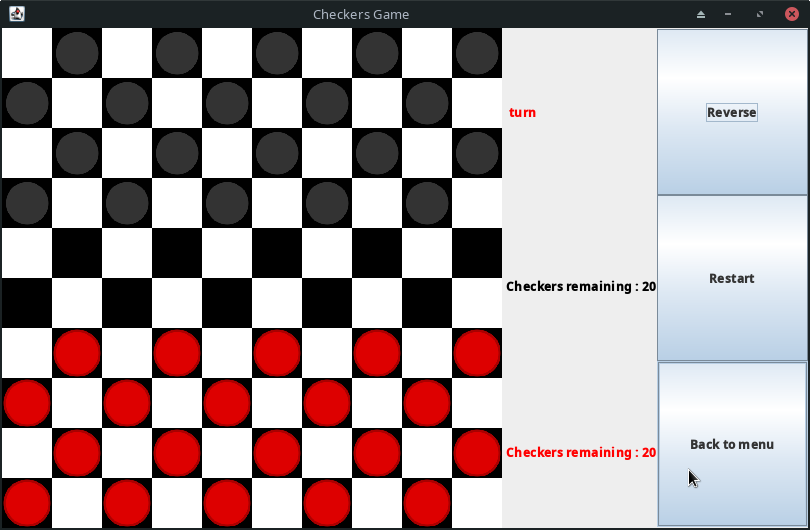
\includegraphics[width=1\columnwidth]{figures/boardGame.png}
    \caption[Fenêtre de jeu]{Fenêtre de jeu}
    \label{f:fenetrePrincipale}
\end{figure}

Pour pouvoir jouer, le joueur doit cliquer sur la pièce qu'il souhaite déplacer. Ensuite,
le joueur doit cliquer sur la ou les cases de destination indiquée avec une couleur jaune
(cf. \hyperref[f:fenetreClick]{figure \ref{f:fenetreClick}}).

\begin{figure}[H]
    \centering
    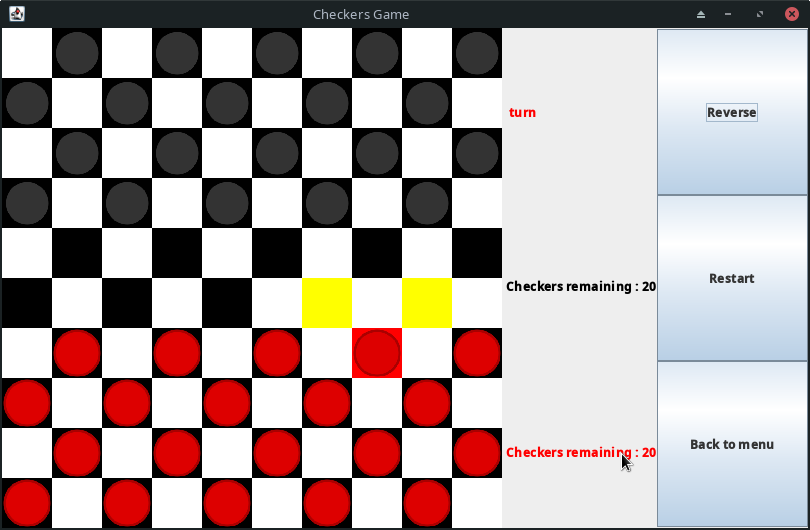
\includegraphics[width=1\columnwidth]{figures/boardGameClick.png}
    \caption[Fenêtre de jeu lorsqu'un joueur clique sur une pièce]{Fenêtre de jeu lorsqu'un joueur clique sur une pièce}
    \label{f:fenetreClick}
\end{figure}

Ensuite, le tour de chaque joueur est fait automatiquement et est indiqué par un message de couleur noir ou rouge 
avec les statistiques.

\section{Logique MVC}

Nous avons décidé de définir un contrôleur \textbf{GameController} qui gère le fonctionnement de l'application.
Ce controleur permet la gestion des entités du jeu (game, board)  et la gestion de l'affichage (boardView). \medskip

Ensuite, pour les vues, nous avons décidé de définir une vue \textbf{Board} qui défini le damier. 
Une autre vue \textbf{Coordinates} qui défini les coordonnées des pièces. 
Puis, une vue \textbf{Game} qui défini le fonctionnement des joueurs pour la partie. 
Pour finir, une vue \textbf{Pawn} qui défini les pièces et une vue \textbf{Player} qui 
défini un joueur. \medskip

Pour finir, au niveau des vues, nous avons décidé de définir une vue \textbf{BoardView} qui affiche le damier 
et qui gère les statistiques. De plus, nous avons aussi une vue \textbf{GridView} 
qui permet de gérer l'affichage du damier. Enfin, une vue \textbf{MenuView} pour afficher 
le menu principal avant de commencer le jeu.

\section{Difficultés rencontrées}

Nous avons eu quelques difficultés comme le fait de gérer le MVC avec l'utilisation des méthodes
qui n'était parfois pas possible/compliqué. Aussi, nous avons eu des difficultés pour gérer l'algorithme 
pour proposer au joueur les solutions de déplacement possible.\medskip

Ces différentes difficultés ont été résolues avec du temps et des efforts.
Malheureusement, nous n'avons pas pu réaliser toutes les fonctions demandées comme 
l'ajout de statistiques plus poussés sur le jeu.


\section{Nos choix}

Nous avons décidé de définir une interface graphique pour l'application simple, mais efficace.
Avec par exemple, uniquement deux champs de texte pour les noms des joueurs et un bouton Play pour lancer la partie.\medskip

De plus, pour distinguer les deux joueurs, nous avons mis deux couleurs : rouge et noir.
Ces couleurs sont utilisées pour les différents messages de statistiques pour différentier les joueurs.

\section{Éléments de configuration}

Nous avons décidé de définir des éléments de configuration pour l'application.
Ces éléments de configuration permettent de définir le nombre de pièces par joueur, le nombre de lignes et colonnes du damier, etc.
Ces éléments de configuration sont définis dans des constantes au sein de l'application.

\section{Résultats}

Le menu principal se présente comme la figure suivante :

\begin{figure}[H]
    \centering
    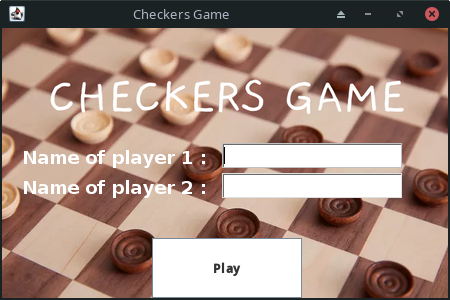
\includegraphics[width=0.8\columnwidth]{figures/mainMenu.png}
    \caption[Menu principal du jeu de dames]{Menu principal du jeu de dames}
    \label{f:menuPrincipall}
\end{figure}

Ensuite, la fenêtre du jeu se présente comme la figure suivante :

\begin{figure}[H]
    \centering
    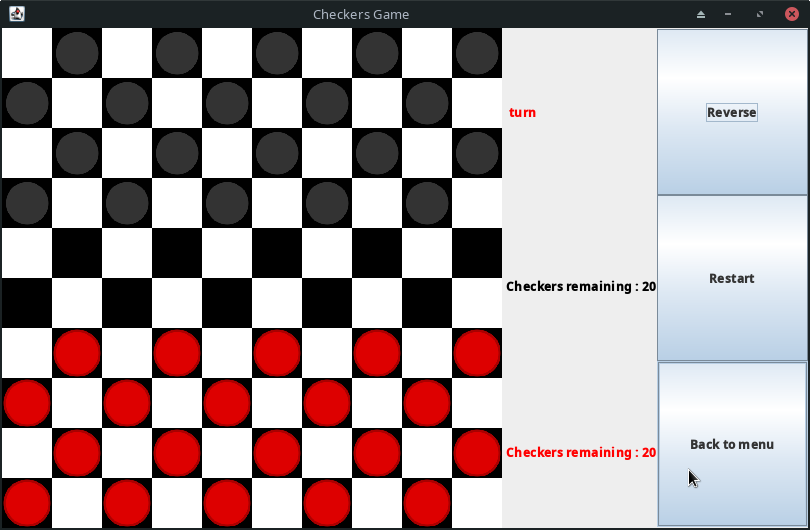
\includegraphics[width=1\columnwidth]{figures/boardGame.png}
    \caption[Fenêtre de jeu]{Fenêtre de jeu}
    \label{f:fenetrePrincipalee}
\end{figure}

Puis une partie de jeu en cours se présente comme la figure suivante :

\begin{figure}[H]
    \centering
    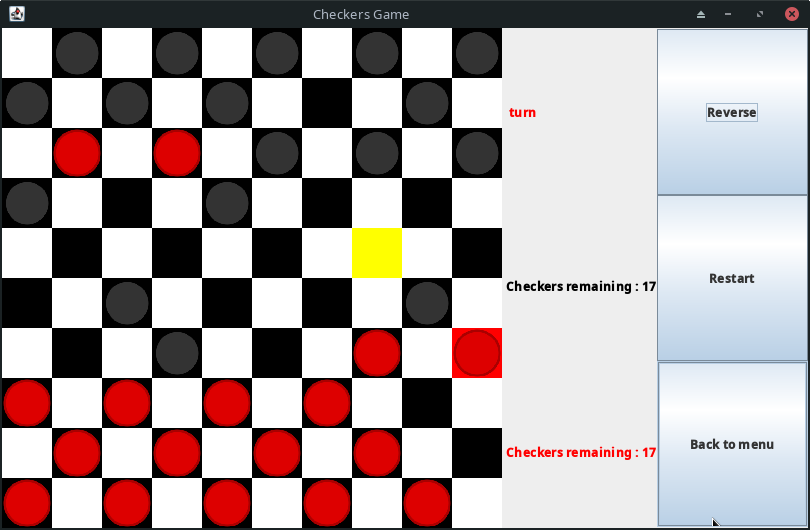
\includegraphics[width=1\columnwidth]{figures/boardGameAdvanced.png}
    \caption[Fenêtre de jeu en cours de partie]{Fenêtre de jeu en cours de partie}
    \label{f:fenetreAvance}
\end{figure}